\documentclass[border=10pt]{standalone}
\usepackage{tikz}
\usepackage[T1]{fontenc}
\usepackage{helvet}
\renewcommand{\familydefault}{\sfdefault}
\usetikzlibrary{arrows.meta,backgrounds}
\definecolor{pr}{HTML}{9E2B2B}
\definecolor{prfill}{HTML}{FBF3F3}
\definecolor{ink}{HTML}{3A3A3A}
\definecolor{mg}{HTML}{6B6B6B}
\definecolor{bg}{HTML}{ADADAD}
\definecolor{bfill}{HTML}{F6F5F3}
\definecolor{edge}{HTML}{CBC7C2}
\definecolor{pg}{HTML}{ABABAB}
\begin{document}
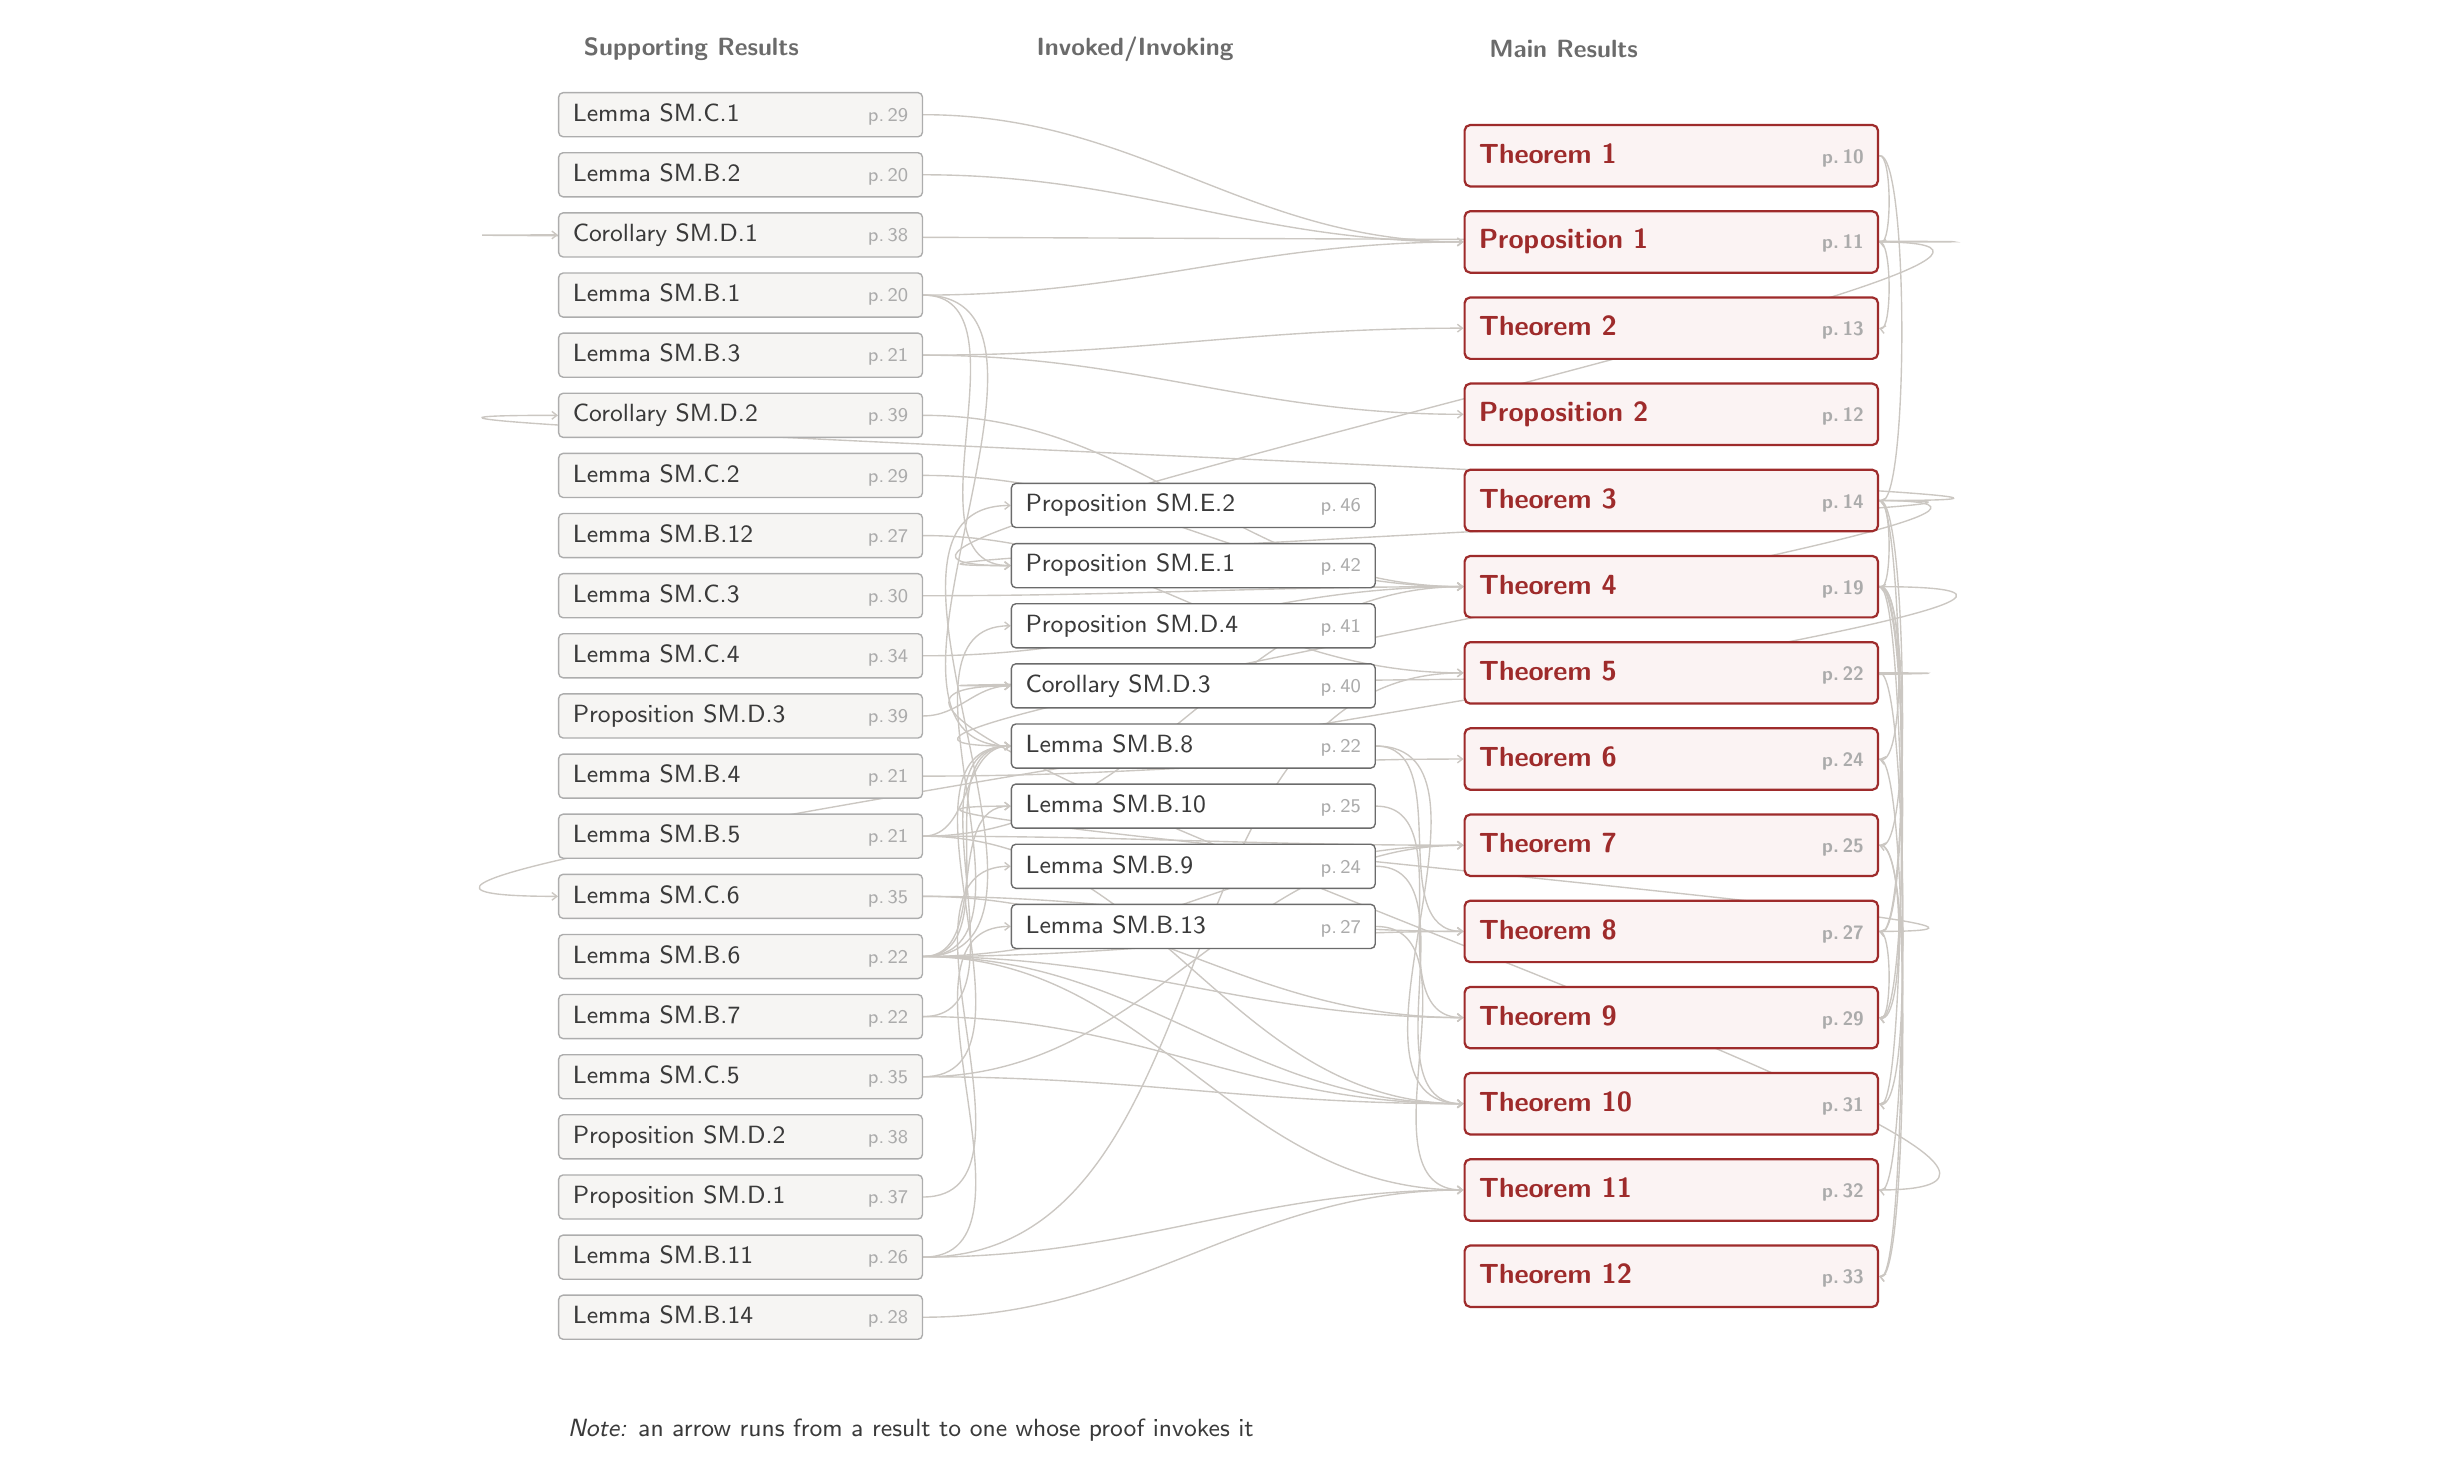
\begin{tikzpicture}[x=1cm,y=1cm,
  main/.style={rounded corners=2pt,draw=pr,fill=prfill,line width=0.8pt,inner sep=0pt,minimum width=5.25cm,minimum height=0.78cm,text=pr,font=\bfseries\normalsize},
  mid/.style={rounded corners=1.6pt,draw=mg,fill=white,line width=0.5pt,inner sep=0pt,minimum width=4.62cm,minimum height=0.56cm,text=ink,font=\small},
  base/.style={rounded corners=1.6pt,draw=bg,fill=bfill,line width=0.5pt,inner sep=0pt,minimum width=4.62cm,minimum height=0.56cm,text=ink,font=\small},
  fl/.style={draw=edge,line width=0.5pt,-{Straight Barb[length=1.8pt,width=2.8pt]}},
]
\node[base,anchor=west] (lemparallel) at (0.000,7.636) {\makebox[4.62cm][l]{\hspace{1.8mm}Lemma SM.C.1\hfill\textcolor{pg}{\scriptsize p.\,29}\hspace{1.8mm}}};
\node[base,anchor=west] (lemlocal) at (0.000,6.873) {\makebox[4.62cm][l]{\hspace{1.8mm}Lemma SM.B.2\hfill\textcolor{pg}{\scriptsize p.\,20}\hspace{1.8mm}}};
\node[base,anchor=west] (coroverlap) at (0.000,6.109) {\makebox[4.62cm][l]{\hspace{1.8mm}Corollary SM.D.1\hfill\textcolor{pg}{\scriptsize p.\,38}\hspace{1.8mm}}};
\node[base,anchor=west] (lemincremental) at (0.000,5.345) {\makebox[4.62cm][l]{\hspace{1.8mm}Lemma SM.B.1\hfill\textcolor{pg}{\scriptsize p.\,20}\hspace{1.8mm}}};
\node[base,anchor=west] (lementry) at (0.000,4.582) {\makebox[4.62cm][l]{\hspace{1.8mm}Lemma SM.B.3\hfill\textcolor{pg}{\scriptsize p.\,21}\hspace{1.8mm}}};
\node[base,anchor=west] (cordegeneracy) at (0.000,3.818) {\makebox[4.62cm][l]{\hspace{1.8mm}Corollary SM.D.2\hfill\textcolor{pg}{\scriptsize p.\,39}\hspace{1.8mm}}};
\node[base,anchor=west] (lemmartingale) at (0.000,3.055) {\makebox[4.62cm][l]{\hspace{1.8mm}Lemma SM.C.2\hfill\textcolor{pg}{\scriptsize p.\,29}\hspace{1.8mm}}};
\node[base,anchor=west] (lemrestricted) at (0.000,2.291) {\makebox[4.62cm][l]{\hspace{1.8mm}Lemma SM.B.12\hfill\textcolor{pg}{\scriptsize p.\,27}\hspace{1.8mm}}};
\node[base,anchor=west] (lemconcentration) at (0.000,1.527) {\makebox[4.62cm][l]{\hspace{1.8mm}Lemma SM.C.3\hfill\textcolor{pg}{\scriptsize p.\,30}\hspace{1.8mm}}};
\node[base,anchor=west] (lemmultilinear) at (0.000,0.764) {\makebox[4.62cm][l]{\hspace{1.8mm}Lemma SM.C.4\hfill\textcolor{pg}{\scriptsize p.\,34}\hspace{1.8mm}}};
\node[base,anchor=west] (propthreeseq) at (0.000,0.000) {\makebox[4.62cm][l]{\hspace{1.8mm}Proposition SM.D.3\hfill\textcolor{pg}{\scriptsize p.\,39}\hspace{1.8mm}}};
\node[base,anchor=west] (lempihat) at (0.000,-0.764) {\makebox[4.62cm][l]{\hspace{1.8mm}Lemma SM.B.4\hfill\textcolor{pg}{\scriptsize p.\,21}\hspace{1.8mm}}};
\node[base,anchor=west] (lemfourth) at (0.000,-1.527) {\makebox[4.62cm][l]{\hspace{1.8mm}Lemma SM.B.5\hfill\textcolor{pg}{\scriptsize p.\,21}\hspace{1.8mm}}};
\node[base,anchor=west] (lemquadformE2) at (0.000,-2.291) {\makebox[4.62cm][l]{\hspace{1.8mm}Lemma SM.C.6\hfill\textcolor{pg}{\scriptsize p.\,35}\hspace{1.8mm}}};
\node[base,anchor=west] (lemleverageid) at (0.000,-3.055) {\makebox[4.62cm][l]{\hspace{1.8mm}Lemma SM.B.6\hfill\textcolor{pg}{\scriptsize p.\,22}\hspace{1.8mm}}};
\node[base,anchor=west] (lemie) at (0.000,-3.818) {\makebox[4.62cm][l]{\hspace{1.8mm}Lemma SM.B.7\hfill\textcolor{pg}{\scriptsize p.\,22}\hspace{1.8mm}}};
\node[base,anchor=west] (lemquadform) at (0.000,-4.582) {\makebox[4.62cm][l]{\hspace{1.8mm}Lemma SM.C.5\hfill\textcolor{pg}{\scriptsize p.\,35}\hspace{1.8mm}}};
\node[base,anchor=west] (lemleverage) at (0.000,-5.345) {\makebox[4.62cm][l]{\hspace{1.8mm}Proposition SM.D.2\hfill\textcolor{pg}{\scriptsize p.\,38}\hspace{1.8mm}}};
\node[base,anchor=west] (propdesigncond) at (0.000,-6.109) {\makebox[4.62cm][l]{\hspace{1.8mm}Proposition SM.D.1\hfill\textcolor{pg}{\scriptsize p.\,37}\hspace{1.8mm}}};
\node[base,anchor=west] (lemsharing) at (0.000,-6.873) {\makebox[4.62cm][l]{\hspace{1.8mm}Lemma SM.B.11\hfill\textcolor{pg}{\scriptsize p.\,26}\hspace{1.8mm}}};
\node[base,anchor=west] (lemsqrt) at (0.000,-7.636) {\makebox[4.62cm][l]{\hspace{1.8mm}Lemma SM.B.14\hfill\textcolor{pg}{\scriptsize p.\,28}\hspace{1.8mm}}};
\node[mid,anchor=west] (propgroupcompute) at (5.750,2.673) {\makebox[4.62cm][l]{\hspace{1.8mm}Proposition SM.E.2\hfill\textcolor{pg}{\scriptsize p.\,46}\hspace{1.8mm}}};
\node[mid,anchor=west] (propcompute) at (5.750,1.909) {\makebox[4.62cm][l]{\hspace{1.8mm}Proposition SM.E.1\hfill\textcolor{pg}{\scriptsize p.\,42}\hspace{1.8mm}}};
\node[mid,anchor=west] (proplc) at (5.750,1.145) {\makebox[4.62cm][l]{\hspace{1.8mm}Proposition SM.D.4\hfill\textcolor{pg}{\scriptsize p.\,41}\hspace{1.8mm}}};
\node[mid,anchor=west] (corclustershock) at (5.750,0.382) {\makebox[4.62cm][l]{\hspace{1.8mm}Corollary SM.D.3\hfill\textcolor{pg}{\scriptsize p.\,40}\hspace{1.8mm}}};
\node[mid,anchor=west] (lemcgm) at (5.750,-0.382) {\makebox[4.62cm][l]{\hspace{1.8mm}Lemma SM.B.8\hfill\textcolor{pg}{\scriptsize p.\,22}\hspace{1.8mm}}};
\node[mid,anchor=west] (lemidentE2) at (5.750,-1.145) {\makebox[4.62cm][l]{\hspace{1.8mm}Lemma SM.B.10\hfill\textcolor{pg}{\scriptsize p.\,25}\hspace{1.8mm}}};
\node[mid,anchor=west] (lemcgmsharp) at (5.750,-1.909) {\makebox[4.62cm][l]{\hspace{1.8mm}Lemma SM.B.9\hfill\textcolor{pg}{\scriptsize p.\,24}\hspace{1.8mm}}};
\node[mid,anchor=west] (leminfeasiblemeat) at (5.750,-2.673) {\makebox[4.62cm][l]{\hspace{1.8mm}Lemma SM.B.13\hfill\textcolor{pg}{\scriptsize p.\,27}\hspace{1.8mm}}};
\node[main,anchor=west] (thmspanning) at (11.500,7.115) {\makebox[5.25cm][l]{\hspace{1.8mm}Theorem 1\hfill\textcolor{pg}{\scriptsize p.\,10}\hspace{1.8mm}}};
\node[main,anchor=west] (propdw) at (11.500,6.020) {\makebox[5.25cm][l]{\hspace{1.8mm}Proposition 1\hfill\textcolor{pg}{\scriptsize p.\,11}\hspace{1.8mm}}};
\node[main,anchor=west] (thmproportional) at (11.500,4.925) {\makebox[5.25cm][l]{\hspace{1.8mm}Theorem 2\hfill\textcolor{pg}{\scriptsize p.\,13}\hspace{1.8mm}}};
\node[main,anchor=west] (proppairwise) at (11.500,3.831) {\makebox[5.25cm][l]{\hspace{1.8mm}Proposition 2\hfill\textcolor{pg}{\scriptsize p.\,12}\hspace{1.8mm}}};
\node[main,anchor=west] (thmjm) at (11.500,2.736) {\makebox[5.25cm][l]{\hspace{1.8mm}Theorem 3\hfill\textcolor{pg}{\scriptsize p.\,14}\hspace{1.8mm}}};
\node[main,anchor=west] (thmclt) at (11.500,1.642) {\makebox[5.25cm][l]{\hspace{1.8mm}Theorem 4\hfill\textcolor{pg}{\scriptsize p.\,19}\hspace{1.8mm}}};
\node[main,anchor=west] (thmcltcluster) at (11.500,0.547) {\makebox[5.25cm][l]{\hspace{1.8mm}Theorem 5\hfill\textcolor{pg}{\scriptsize p.\,22}\hspace{1.8mm}}};
\node[main,anchor=west] (thmpi) at (11.500,-0.547) {\makebox[5.25cm][l]{\hspace{1.8mm}Theorem 6\hfill\textcolor{pg}{\scriptsize p.\,24}\hspace{1.8mm}}};
\node[main,anchor=west] (thmvhat) at (11.500,-1.642) {\makebox[5.25cm][l]{\hspace{1.8mm}Theorem 7\hfill\textcolor{pg}{\scriptsize p.\,25}\hspace{1.8mm}}};
\node[main,anchor=west] (thmunionmeat) at (11.500,-2.736) {\makebox[5.25cm][l]{\hspace{1.8mm}Theorem 8\hfill\textcolor{pg}{\scriptsize p.\,27}\hspace{1.8mm}}};
\node[main,anchor=west] (thmplugin) at (11.500,-3.831) {\makebox[5.25cm][l]{\hspace{1.8mm}Theorem 9\hfill\textcolor{pg}{\scriptsize p.\,29}\hspace{1.8mm}}};
\node[main,anchor=west] (thmabsorbed) at (11.500,-4.925) {\makebox[5.25cm][l]{\hspace{1.8mm}Theorem 10\hfill\textcolor{pg}{\scriptsize p.\,31}\hspace{1.8mm}}};
\node[main,anchor=west] (thmrateagnostic) at (11.500,-6.020) {\makebox[5.25cm][l]{\hspace{1.8mm}Theorem 11\hfill\textcolor{pg}{\scriptsize p.\,32}\hspace{1.8mm}}};
\node[main,anchor=west] (thmpiinf) at (11.500,-7.115) {\makebox[5.25cm][l]{\hspace{1.8mm}Theorem 12\hfill\textcolor{pg}{\scriptsize p.\,33}\hspace{1.8mm}}};
\begin{scope}[on background layer]
\draw[fl] (cordegeneracy.east) to[out=0,in=180] (thmclt.west);
\draw[fl] (lemcgm.east) to[out=0,in=180] (thmabsorbed.west);
\draw[fl] (lemcgm.east) to[out=0,in=180] (thmunionmeat.west);
\draw[fl] (lemcgmsharp.east) to[out=0,in=180] (thmabsorbed.west);
\draw[fl] (lemconcentration.east) to[out=0,in=180] (thmclt.west);
\draw[fl] (lementry.east) to[out=0,in=180] (proppairwise.west);
\draw[fl] (lementry.east) to[out=0,in=180] (thmproportional.west);
\draw[fl] (lemfourth.east) to[out=0,in=180] (lemcgm.west);
\draw[fl] (lemfourth.east) to[out=0,in=180] (thmabsorbed.west);
\draw[fl] (lemfourth.east) to[out=0,in=180] (thmclt.west);
\draw[fl] (lemfourth.east) to[out=0,in=180] (thmvhat.west);
\draw[fl] (lemidentE2.east) to[out=0,in=180] (thmplugin.west);
\draw[fl] (lemie.east) to[out=0,in=180] (lemcgm.west);
\draw[fl] (lemie.east) to[out=0,in=180] (thmabsorbed.west);
\draw[fl] (lemincremental.east) to[out=0,in=180] (lemcgm.west);
\draw[fl] (lemincremental.east) to[out=0,in=180] (propcompute.west);
\draw[fl] (lemincremental.east) to[out=0,in=180] (propdw.west);
\draw[fl] (leminfeasiblemeat.east) to[out=0,in=180] (thmrateagnostic.west);
\draw[fl] (lemleverageid.east) to[out=0,in=180] (lemcgm.west);
\draw[fl] (lemleverageid.east) to[out=0,in=180] (lemidentE2.west);
\draw[fl] (lemleverageid.east) to[out=0,in=180] (propgroupcompute.west);
\draw[fl] (lemleverageid.east) to[out=0,in=180] (proplc.west);
\draw[fl] (lemleverageid.east) to[out=0,in=180] (thmabsorbed.west);
\draw[fl] (lemleverageid.east) to[out=0,in=180] (thmplugin.west);
\draw[fl] (lemleverageid.east) to[out=0,in=180] (thmrateagnostic.west);
\draw[fl] (lemleverageid.east) to[out=0,in=180] (thmunionmeat.west);
\draw[fl] (lemleverageid.east) to[out=0,in=180] (thmvhat.west);
\draw[fl] (lemlocal.east) to[out=0,in=180] (propdw.west);
\draw[fl] (lemmartingale.east) to[out=0,in=180] (thmclt.west);
\draw[fl] (lemmultilinear.east) to[out=0,in=180] (thmclt.west);
\draw[fl] (lemparallel.east) to[out=0,in=180] (propdw.west);
\draw[fl] (lempihat.east) to[out=0,in=180] (thmpi.west);
\draw[fl] (lemquadform.east) to[out=0,in=180] (lemcgm.west);
\draw[fl] (lemquadform.east) to[out=0,in=180] (thmabsorbed.west);
\draw[fl] (lemquadform.east) to[out=0,in=180] (thmvhat.west);
\draw[fl] (lemquadformE2.east) to[out=0,in=180] (thmplugin.west);
\draw[fl] (lemquadformE2.east) to[out=0,in=180] (thmunionmeat.west);
\draw[fl] (lemrestricted.east) to[out=0,in=180] (thmcltcluster.west);
\draw[fl] (lemsharing.east) to[out=0,in=180] (leminfeasiblemeat.west);
\draw[fl] (lemsharing.east) to[out=0,in=180] (thmcltcluster.west);
\draw[fl] (lemsharing.east) to[out=0,in=180] (thmrateagnostic.west);
\draw[fl] (lemsqrt.east) to[out=0,in=180] (thmrateagnostic.west);
\draw[fl] (propdesigncond.east) to[out=0,in=180] (lemcgmsharp.west);
\draw[fl] (propdw.east) to[out=0,in=180] (coroverlap.west);
\draw[fl] (propdw.east) to[out=0,in=180] (propcompute.west);
\draw[fl] (propdw.east) to[out=14,in=-14,looseness=0.40] (thmproportional.east);
\draw[fl] (propthreeseq.east) to[out=0,in=180] (corclustershock.west);
\draw[fl] (thmclt.east) to[out=0,in=180] (lemquadformE2.west);
\draw[fl] (thmclt.east) to[out=14,in=-14,looseness=0.40] (thmpi.east);
\draw[fl] (thmclt.east) to[out=14,in=-14,looseness=0.12] (thmpiinf.east);
\draw[fl] (thmclt.east) to[out=14,in=-14,looseness=0.19] (thmplugin.east);
\draw[fl] (thmclt.east) to[out=14,in=-14,looseness=0.23] (thmunionmeat.east);
\draw[fl] (thmclt.east) to[out=14,in=-14,looseness=0.31] (thmvhat.east);
\draw[fl] (thmcltcluster.east) to[out=0,in=180] (corclustershock.west);
\draw[fl] (thmcltcluster.east) to[out=14,in=-14,looseness=0.16] (thmrateagnostic.east);
\draw[fl] (thmjm.east) to[out=0,in=180] (cordegeneracy.west);
\draw[fl] (thmjm.east) to[out=0,in=180] (lemcgm.west);
\draw[fl] (thmjm.east) to[out=0,in=180] (propcompute.west);
\draw[fl] (thmjm.east) to[out=14,in=-14,looseness=0.13] (thmabsorbed.east);
\draw[fl] (thmjm.east) to[out=14,in=-14,looseness=0.40] (thmclt.east);
\draw[fl] (thmjm.east) to[out=14,in=-14,looseness=0.19] (thmunionmeat.east);
\draw[fl] (thmpi.east) to[out=14,in=-14,looseness=0.16] (thmpiinf.east);
\draw[fl] (thmrateagnostic.east) to[out=0,in=180] (corclustershock.west);
\draw[fl] (thmspanning.east) to[out=14,in=-14,looseness=0.40] (propdw.east);
\draw[fl] (thmspanning.east) to[out=14,in=-14,looseness=0.23] (thmjm.east);
\draw[fl] (thmunionmeat.east) to[out=0,in=180] (lemidentE2.west);
\draw[fl] (thmunionmeat.east) to[out=14,in=-14,looseness=0.40] (thmplugin.east);
\draw[fl] (thmvhat.east) to[out=14,in=-14,looseness=0.31] (thmabsorbed.east);
\draw[fl] (thmvhat.east) to[out=14,in=-14,looseness=0.40] (thmplugin.east);
\end{scope}
\node[anchor=west,font=\bfseries\small,text=mg] at (0.205,8.466) {Supporting Results};
\node[anchor=west,font=\bfseries\small,text=mg] at (5.955,8.466) {Invoked/Invoking};
\node[anchor=west,font=\bfseries\small,text=mg] at (11.705,8.466) {Main Results};
\node[anchor=west,font=\small,text=ink] at (0,-9.066) {\textit{Note:} an arrow runs from a result to one whose proof invokes it};
\end{tikzpicture}
\end{document}
